%----------------------------------------------------------------------------------------
%	OPACITY METHODS
%----------------------------------------------------------------------------------------
%\section{Opacity derivation}
%\label{se:opacities}
%
% LP: copie de l'intro de Xavier
In NIKA2, the opacity is measured via a total-power technique, which was successfully tested with NIKA. The details of this technique and its agreement with the Atmospheric Transmission at Microwaves (ATM) model (\cite{2001IEEE....49.1683C}) are described in \cite{Catalano2014}. The underlying idea is to replace the opacity, usually delivered by the resident IRAM tau-meter that performs elevation scans at a fixed azimuth and is operating at 225\,GHz, by a measurement that uses the NIKA2 instrument itself as a tau-meter. Using this procedure we can directly derive an opacity integrated in the NIKA2 very bandpasses and in the same line-of-sight of the source in the considered map. First, we have to calibrate the relationship between total power and opacity.
% fin copie

\subsection{Methodology}
For each kid $k$, the absolute value of the resonance frequency
$f_{tone}^k$ moves with the atmospheric load according to

\begin{equation}
f_{tone}^k = C_0^k + C_1^k T_{atm}[1-e^{-\tau/\sin\delta}]
\end{equation}

{\bf LP: pourquoi signe plus alors qu'on utilise un signe moins dans
  Eq. 2 du papier instru ?}

where $C_0^k$ is a constant equal to the resonance
frequency at zero opacity, $C_1^k$ is the calibration conversion
factor in kHz$/$K, $T_{atm}$ is the equivalent temperature
of the atmosphere (taken as a constant at 270K), $\tau$ the zenith
opacity and $\delta$ the average elevation of the telescope.
By assuming a homogeneous plane-parallel atmosphere, the airmass $x$ is defined from the
elevation as $x = \sin\delta$. 

The coefficients $C_0^k$ and $C_1^k$ are expected to be constant in time
within at least a cooldown cycle, and are determined using a {\tt
  skydip} procedure. This consists in moving
the telescope in elevation step by step and to monitor, for each kid, the
evolution of $f_{tone}^k$ vs the air mass and to fit the zenith opacity $\tau$ and
$C_0^k$ and $C_1^k$. Namely, during a {\tt skydip}, the telescope performs
eleven elevation steps in the elevation range from 19 to 65 degrees, regularly
spaced in airmass. For each step, we acquire about twenty seconds of
time traces to reduce the error in the determination of $f_{tone}^k$.

All the skydips (that were obtained under various opacity
conditions) are analysed together to break the degeneracies between
the opacity and the responsivity. The procedure has two steps.
First, all the skydips are analysed individually to simply measure
$f_{tone}^k$ for each stable elevation and fit simultaneously all the
parameters ($\tau$, $C_0^k$ and $C_1^k$.)
Error bars on $\tau$ are estimated by doing
this procedure on blocks of 40 kids only and getting a dispersion on the
resulting $\tau$ from the different blocks. Usually the dispersion comes out as
$4\times 10^{-3}$ at 1mm and $1\times 10^{-3}$ at 2mm. Once the $\tau$ values
are estimated for each skydip (as the average over the blocks), we compute
(while fixing $\tau$) the $C_0$ and $C_1$ final values for each KID. We thus
retrieve the coefficients of all the KIDs even though some of them could not
contribute to the tau determination.

%% \begin{figure}
%% \begin{center}
%% 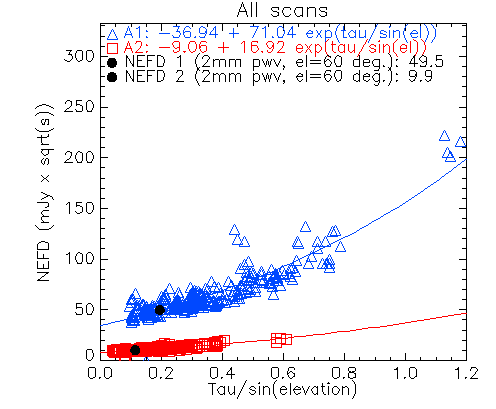
\includegraphics[clip, angle=0, scale =
%%   0.5]{Figures/NEFD_vs_tau_20170226s415_FXDC0C1_Jy_common_mode_kids_out.png}
%% 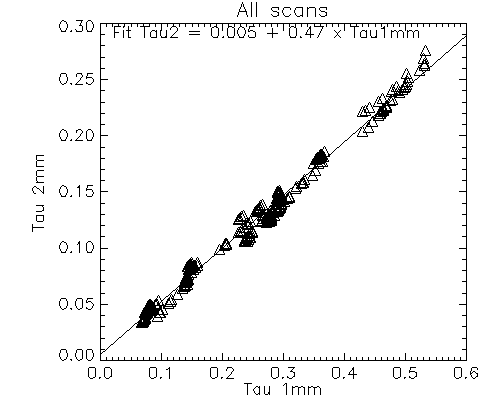
\includegraphics[clip, angle=0, scale =
%%   0.5]{Figures/tau1_tau2_20170226s415_FXDC0C1_GaussPhot_common_mode_kids_out.png}
%% \caption{}
%% \label{fig:fov}
%% \end{center}
%% \end{figure}

%  figure deplacee dans Opacity_checks.tex
%\begin{figure}
%\begin{center}
%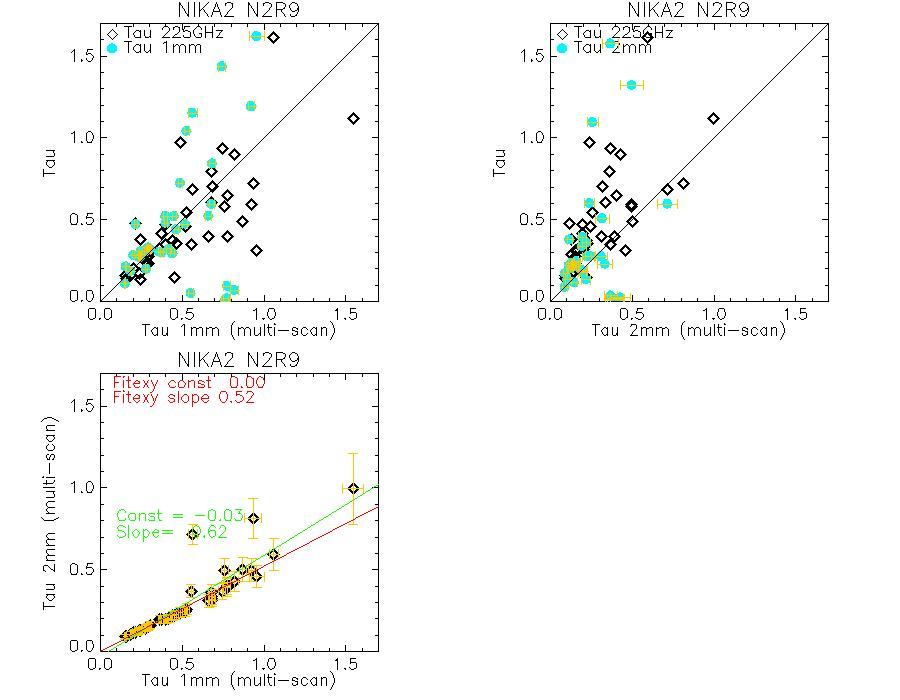
\includegraphics[clip, angle=0, scale = 0.5]{Figures/test_allskd_N2R9.jpg}
%\caption{{\bf Fix me : improve plot quality and plot only the 3rd one.}}
%\label{fig:test_allskd_N2R9}
%\end{center}
%\end{figure}

%\subsection{Opacity measurement consistency tests}

%{\bf copy from the 'Instru' paper}

\begin{figure}[ht]
\begin{center}
\includegraphics[scale=0.8]{Figures/test_allskd_N2R10v2commiss2.pdf}
\caption{Atmospheric opacity as measured from the NIKA2 data 
at 260 (top) and 150\,GHz (bottom) during N2R10
commissioning campaign. Each block of 40 KIDs gives an independent estimate of
the opacity value for each skydip scan (the integer abscissae). The block
number is the decimal value of the abscissae.
\label{fig:taumeas_paper}}
\end{center}
\end{figure}

\begin{figure}[ht]
\begin{center}
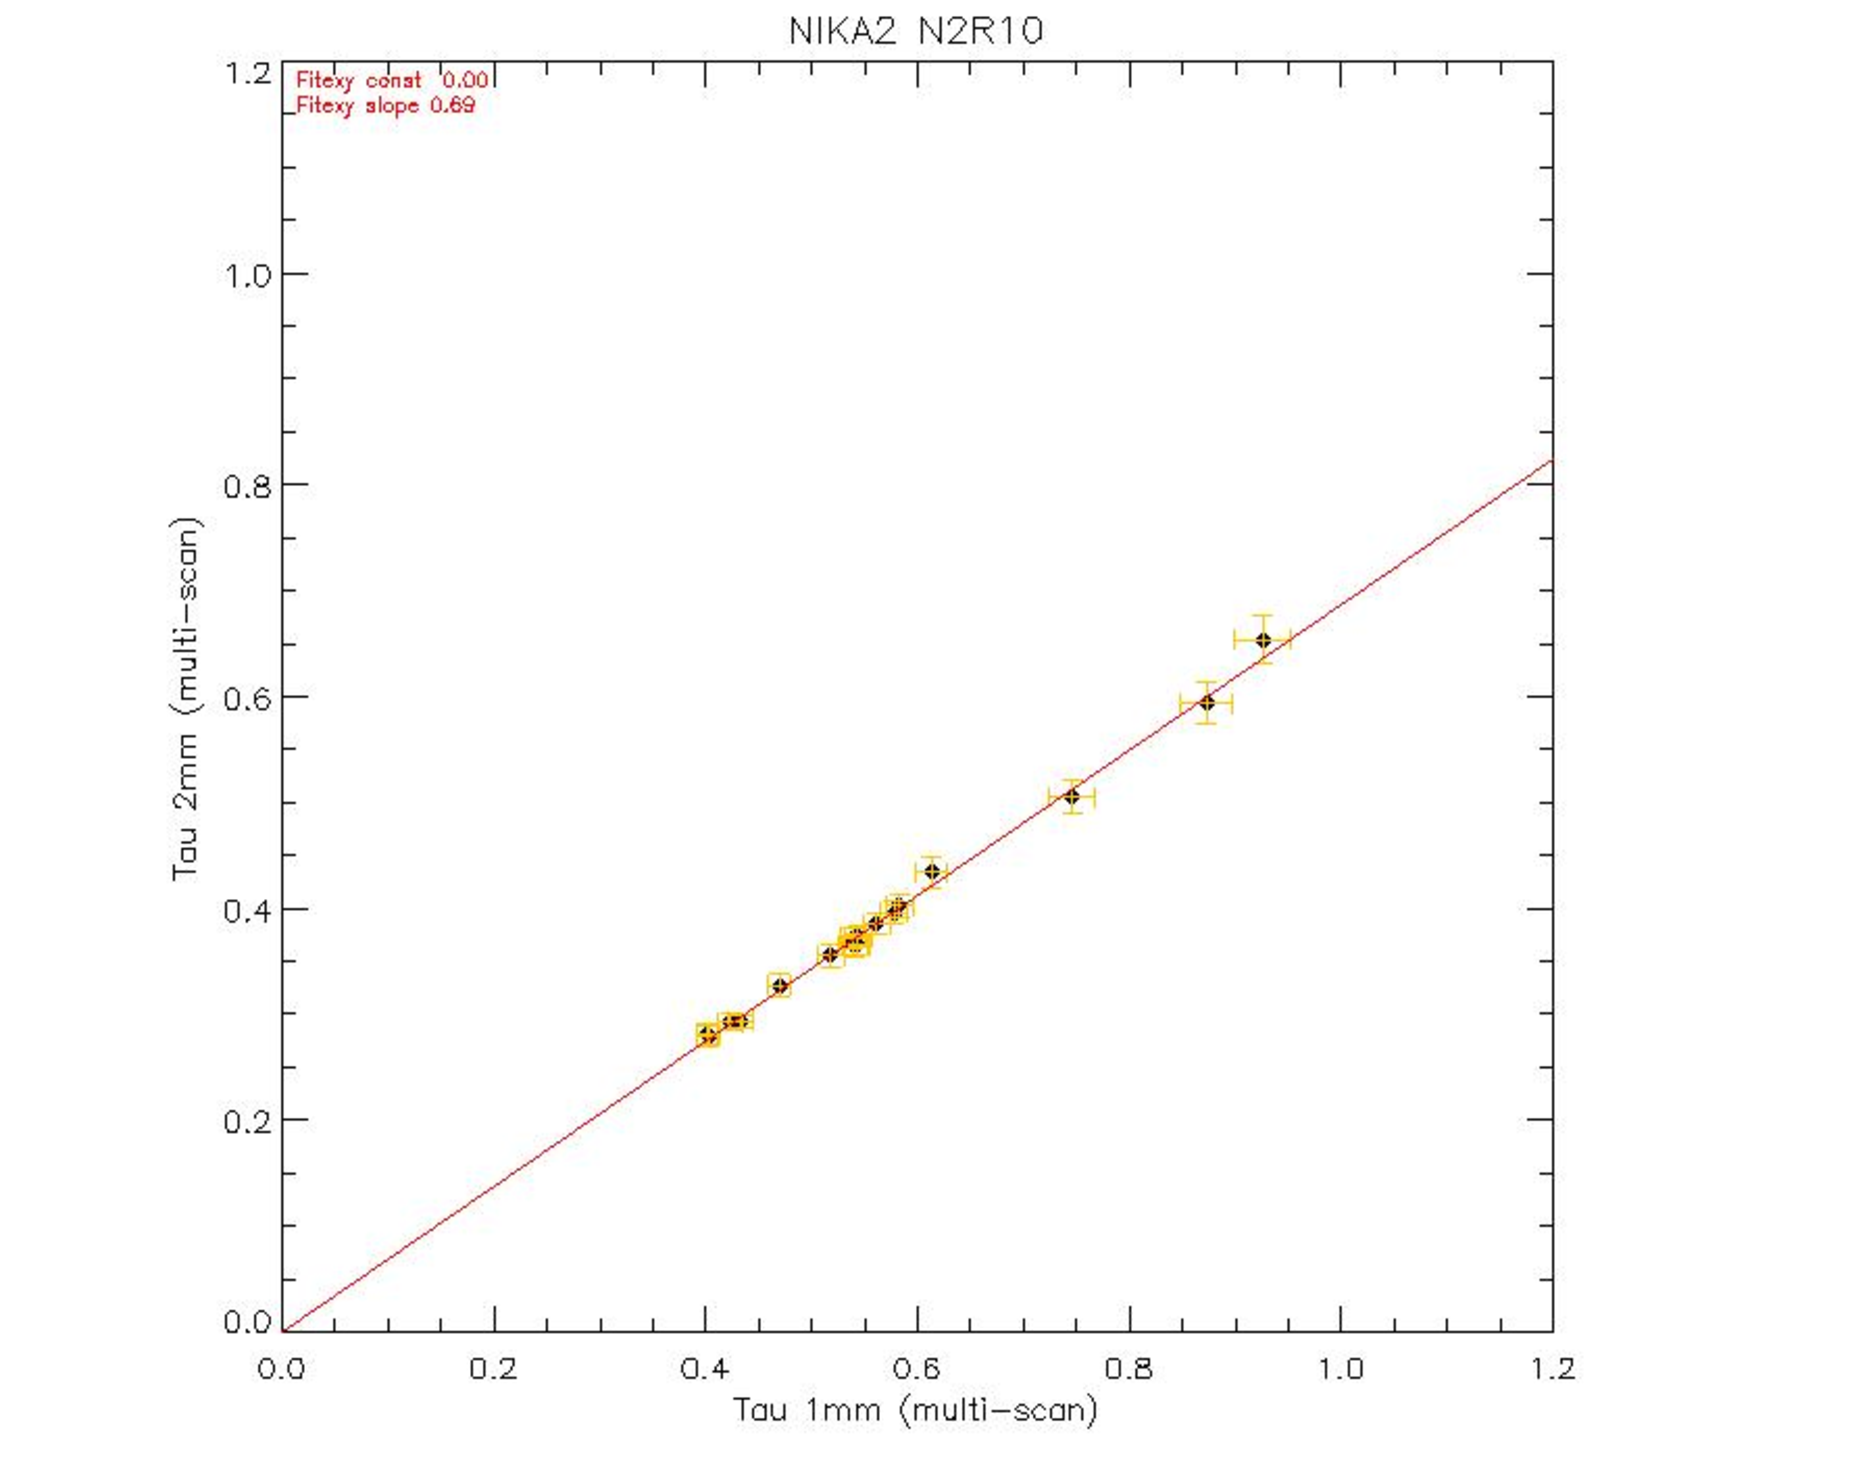
\includegraphics[scale=0.8]{Figures/test_allskd_N2R10v2commiss1.pdf}
\caption{Atmospheric opacity as measured from the NIKA2 data 
at 260 and 150\,GHz during N2R10
commissioning campaign. The error bars are in fact dispersion of the deduced
opacities between blocks of 40 KIDs.
\label{fig:taumeas_paper}}
\end{center}
\end{figure}

We observe that the skydip-fitted $\tau$ values are, as expected, common
between different detectors of the same array (the two 1mm arrays show
slightly different values). By comparing the results of different skydips, we
have verified experimentally that the coefficients $C_0$, $C_1$ are stable,
within the fit errors, on very long time scales within a cooldown cycle. The
coefficients can thus be applied to the whole observing campaign in order to
recover the opacity of each scan.


% \noindent {\bf FM : a figure would help to convince the reader that it is stable on lng time
% scale, which is a key point.}\\ FXD: I will do that figure


\begin{figure}[ht]
\begin{center}
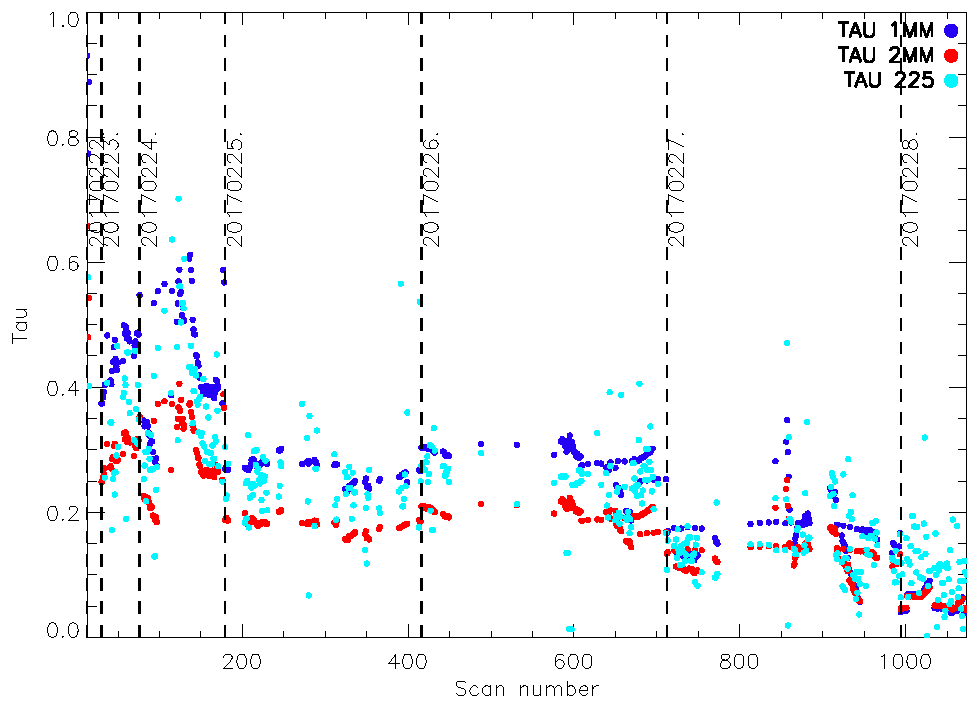
\includegraphics[scale=0.8]{../../Paper_NIKA2_Technical/opacity_evol_run22.pdf}
\caption{Atmospheric opacity as measured from the IRAM 225\,GHz taumeter
(cyan), and from the NIKA2 data at 150 (red) and 260\,GHz (blue) during N2R9
commissioning campaign (Feb. 2017). We stress the fact that the IRAM 225\,GHz
taumeter data is not used for the atmospheric correction and is plotted here
just for comparison.
  \label{fig:taumeas_paper}}
\end{center}
\end{figure}


\begin{figure}[ht]
\begin{center}
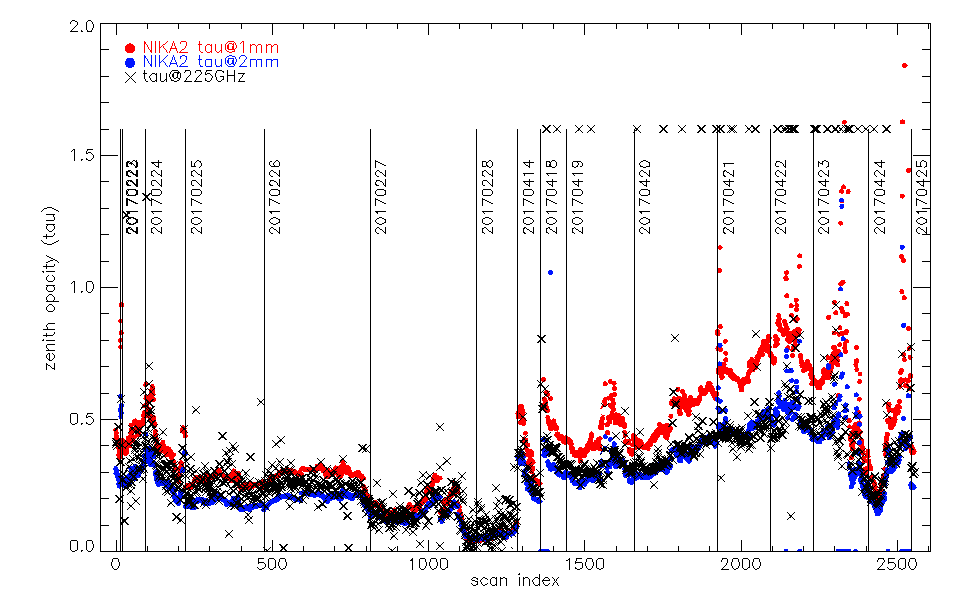
\includegraphics[width=\linewidth]{Figures/opacity_vs_index_N2R9_N2R10.png}
\caption{Atmospheric opacity as measured from the IRAM 225\,GHz
  taumeter (black crosses), and from the NIKA2 data at 150 (red) and 260\,GHz (blue) during 
  N2R9 and N2R10 commissioning campaigns.  We stress the fact that the IRAM 225\,GHz taumeter data is not used for the atmospheric correction and is plotted here just for comparison.
  \label{fig:taumeas}}
\end{center}
\end{figure}


In Fig.~\ref{fig:taumeas} {\bf(and Fig.~\ref{fig:taumeas_paper} of
  \ref{NIKA2-Tech}) } we present the evolution of the NIKA2 in-band
opacities for all the 'OTF' scans (about 1300 scans per runs) of the
N2R9 run held in February and the N2R10 run in April 2017. These are
compared to the IRAM tau-meter values. We observe an agreement on the global trend between the IRAM tau-meter opacity
(225 GHz) and the NIKA2 values. These latter show, however,
a smaller dispersion (less than one percent).
% {\bf FM : how small ?}.


We find an average ratio between the 150 GHz and the 260 GHz NIKA2 values of
about 0.6, a bit higher than ATM model expectations. We notice however that
the 150 GHz-to-260 GHz opacity ratio varies significantly for opacities (at
150 GHz) below 0.2. This effect is likely to be linked to an $O_2$ atmospheric
line which becomes saturated or to some spillover at 2mm. This point is,
however, still under investigation.''


% \noindent {\bf FM : a figure of the ratio of taus would be useful. It should be compared with  
% Fig. \ref{thopacities}, which should appear in this section ...}
% FXD: figure above gives the measured ratio. 


\begin{figure}[ht]
\begin{center}
  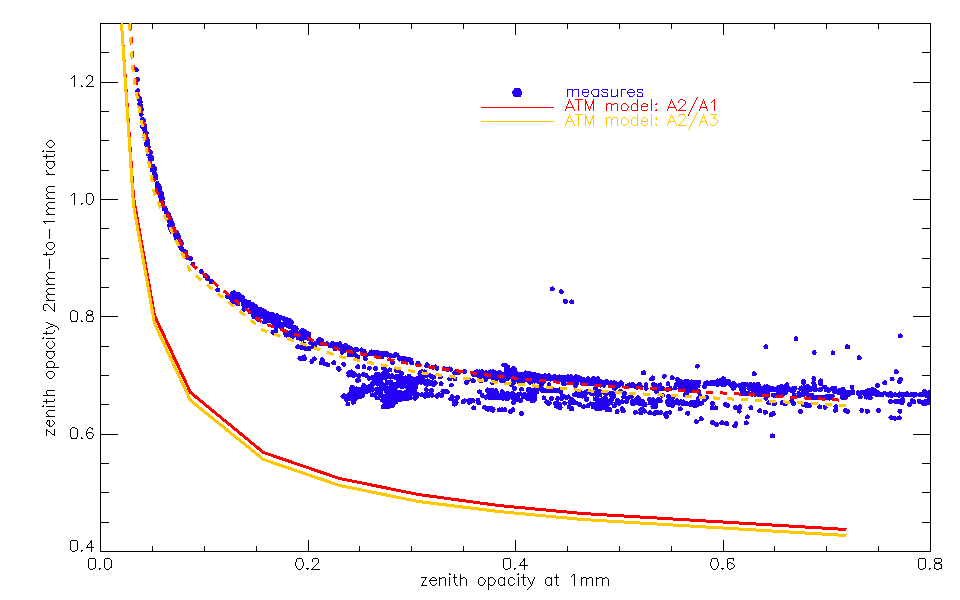
\includegraphics[width=0.65\textwidth]{Figures/opacity_tau1_tau2_ratio_N2R9_N2R10.png}
  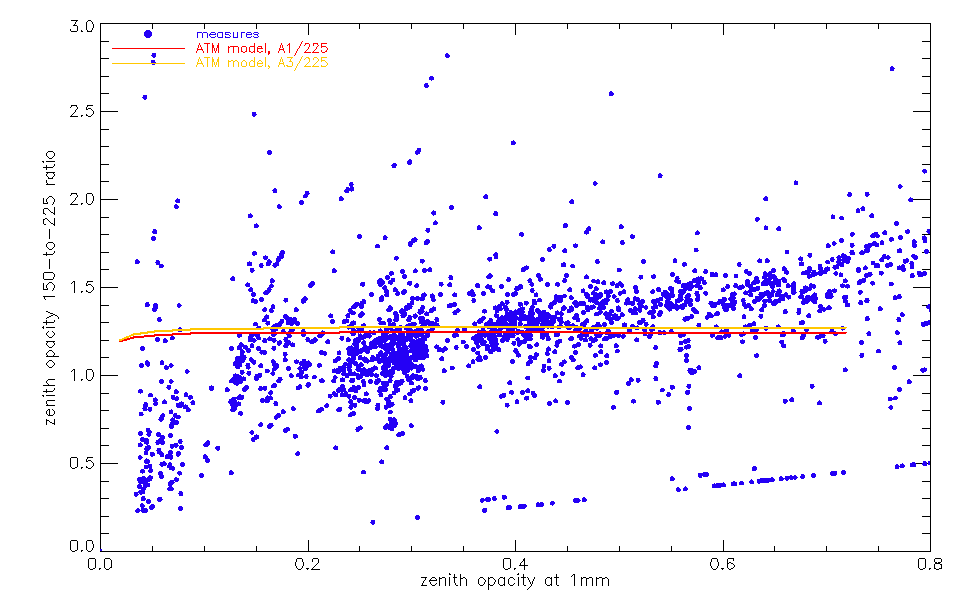
\includegraphics[width=0.65\textwidth]{Figures/opacity_tau1_tau225_ratio_N2R9_N2R10.png}
  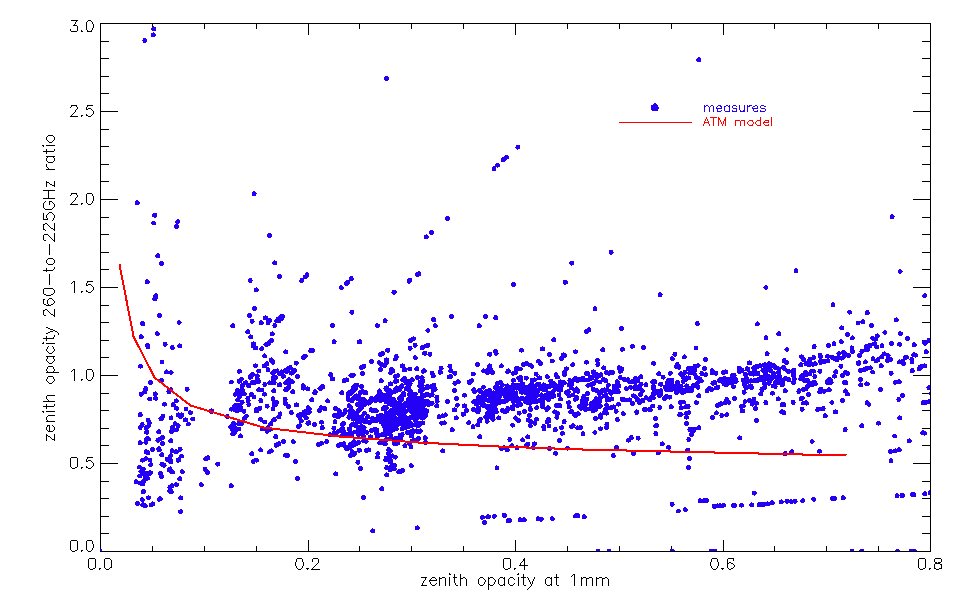
\includegraphics[width=0.65\textwidth]{Figures/opacity_tau2_tau225_ratio_N2R9_N2R10.png}
\caption{Ratios between the 150 GHz and the 260 GHz NIKA2 zenith opacity
estimates and between the NIKA2 $\tau$ and the IRAM taumeter
values. The expectation values derived for NIKA2 bands
using the ATM model described in \ref{Pardo2002} are shown for
comparison (red and orange curves).}
  \label{fig:opacity_ratios}
\end{center}
\end{figure}

\begin{figure}[ht]
\begin{center}
  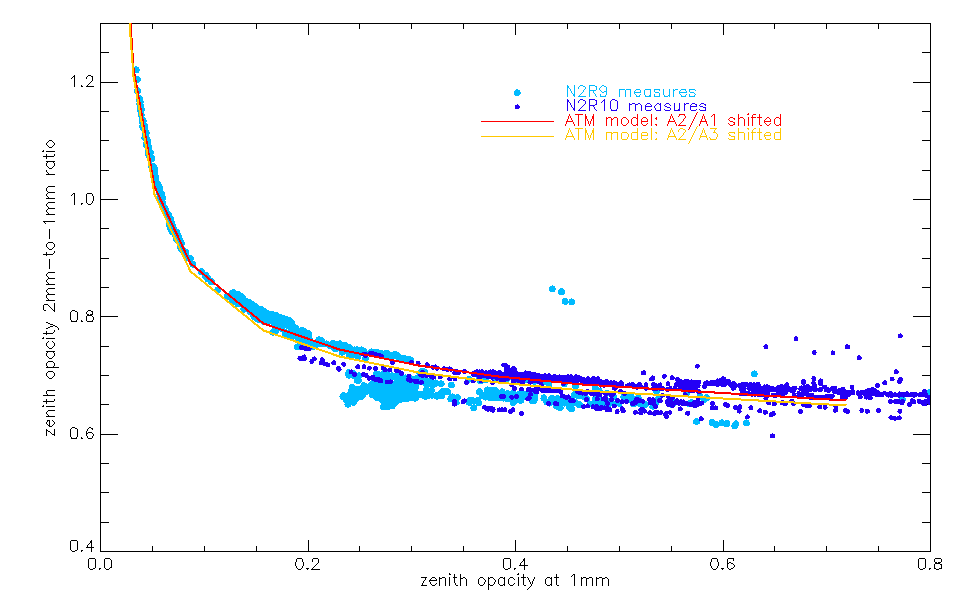
\includegraphics[width=0.8\textwidth]{Figures/opacity_tau1_tau2_byrun_ratio_N2R9_N2R10.png}
  \caption{Ratio between the 150 GHz and the 260 GHz NIKA2 zenith opacity
estimates. The expectation values derived for NIKA2 bands
using the ATM model described in \ref{Pardo2002} are shown for
comparison (red and orange curves). The observed NIKA2 opacity ratio
has a smooth, consistent behaviour over the overall probed opacity range,
and very few outlier estimates are seen although no scan selection has
been performed (out from discarding the dark tests). Also remarkable
is the consistency between estimates obtained during two campaigns
held two months apart in different weather conditions (good to average
during N2R9 and poor and often hightly unstable conditions during
N2R10). Some sub-structures are seen in the opacity ratio, which are
under investigations. They can have several origins (telescope cabin
temperature variation, variation of the $0_2$ fraction, atmospheric
temperature variation, internal temperature variations, etc).  
  }
  \label{fig:opacity_ratio_perrun}
\end{center}
\end{figure}


\begin{figure}[ht]
\begin{center}
  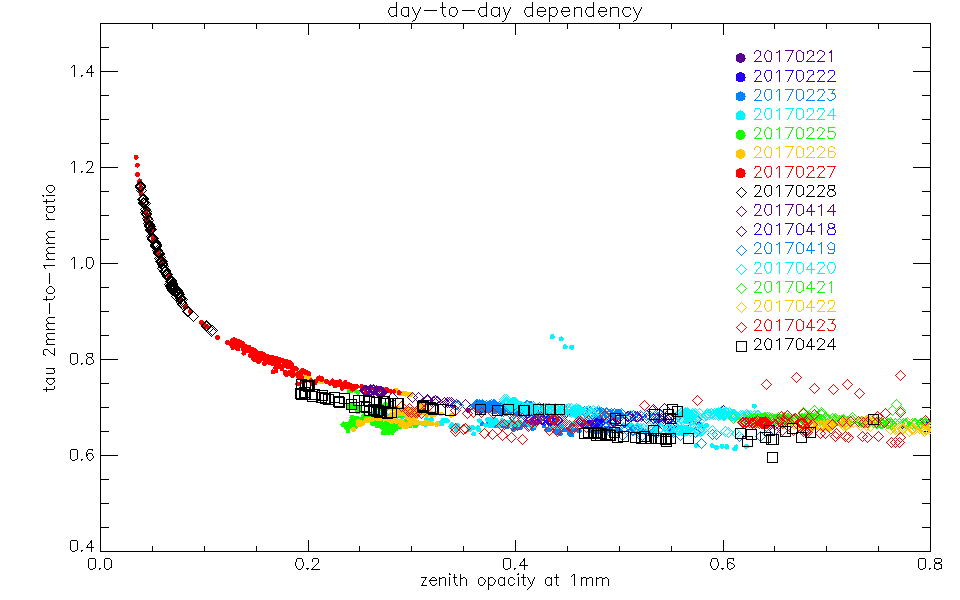
\includegraphics[width=0.8\textwidth]{Figures/opacity_tau1_tau2_ratio_perday_N2R9_N2R10.png}
  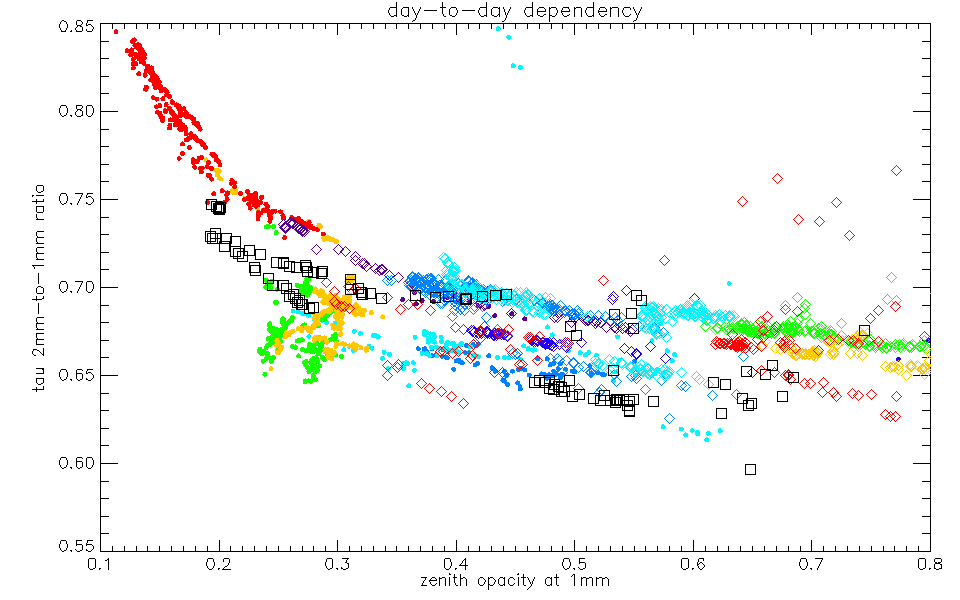
\includegraphics[width=0.8\textwidth]{Figures/opacity_tau1_tau2_ratio_perday_zoom_N2R9_N2R10.png}
  \caption{Ratio between the 150 GHz and the 260 GHz NIKA2 zenith
    opacity estimates. The 4 outlier estimates on February, 24 (in
    cyan) correspond to a test using the external
    calibrator. Different regimes are seen on the 25th and 26th of
    February, while the weather conditions were too unstable to allow
    the astronomer team to focus.
  }
  \label{fig:opacity_ratio_perday}
\end{center}
\end{figure}


\begin{figure}[ht]
\begin{center}
  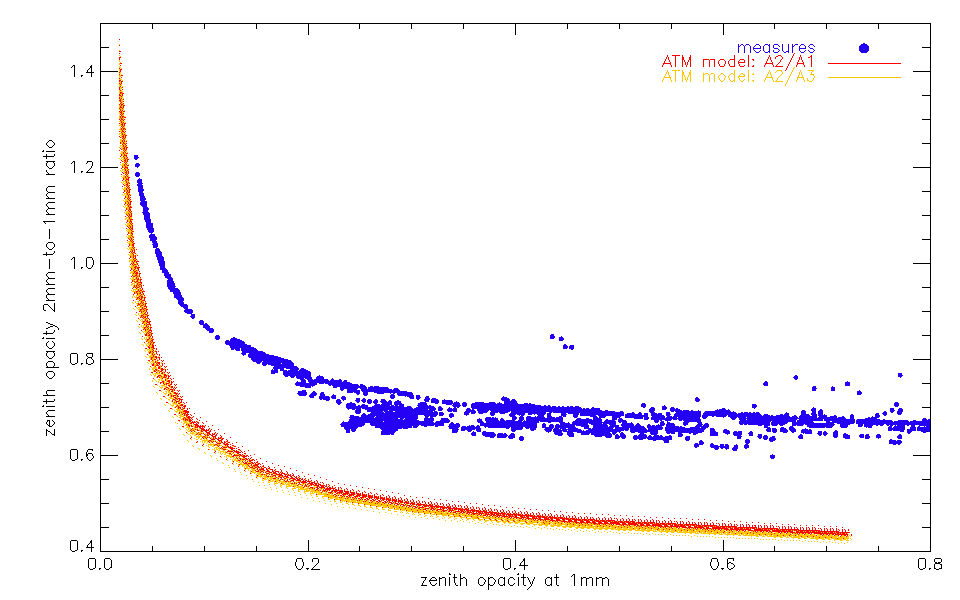
\includegraphics[width=0.8\textwidth]{Figures/opacity_tau1_tau2_ratio_bperror10pc_N2R9_N2R10.png}
  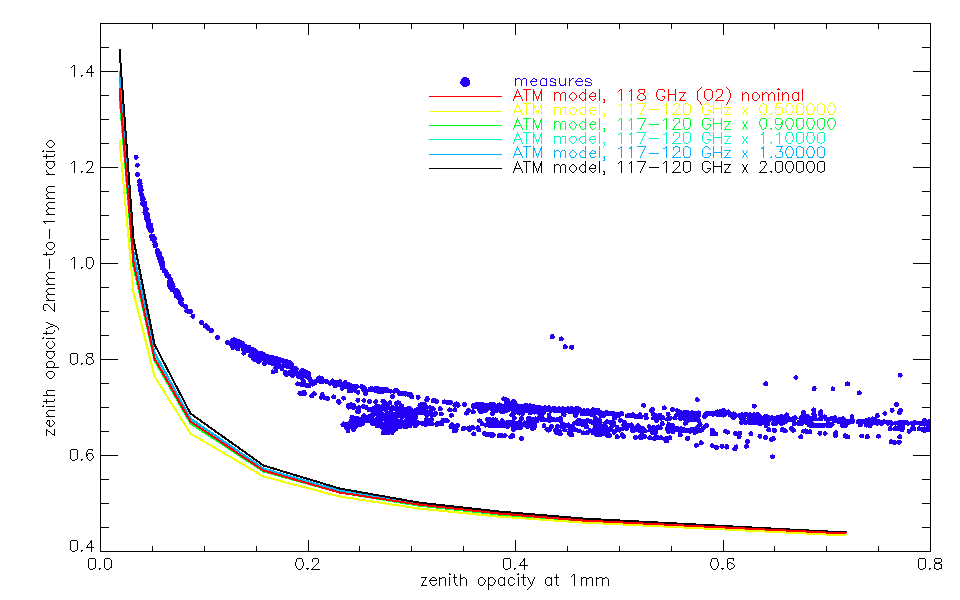
\includegraphics[width=0.8\textwidth]{Figures/opacity_tau1_tau2_ratio_o2fraction_N2R9_N2R10.png}
\caption{Uncertainty of NIKA2 $\tau$ values. Upper panel: The impact
  of the NIKA2 transmission measurement uncertainties is illustrated
  using a very pessimistic relative uncertainty of $10\%$ (instead of
  the more realistic $1\%$ errors). Lower panel: The impact of the
uncertainty on the atmospheric absorption around $118\, \rm{GHz}$, due
to the lack of precise knowledge of the fraction of oxygene in the
atmosphere. The nominal absorption predicted by the ATM model is
modified by a factor from 0.5 to 2 in the $117-120\, \rm{GHz}$
frequency band, where the $0_2$ contributions largely dominates the
water vapor ones. }
  \label{fig:opacity_errors}
\end{center}
\end{figure}

\begin{figure}[ht]
\begin{center}
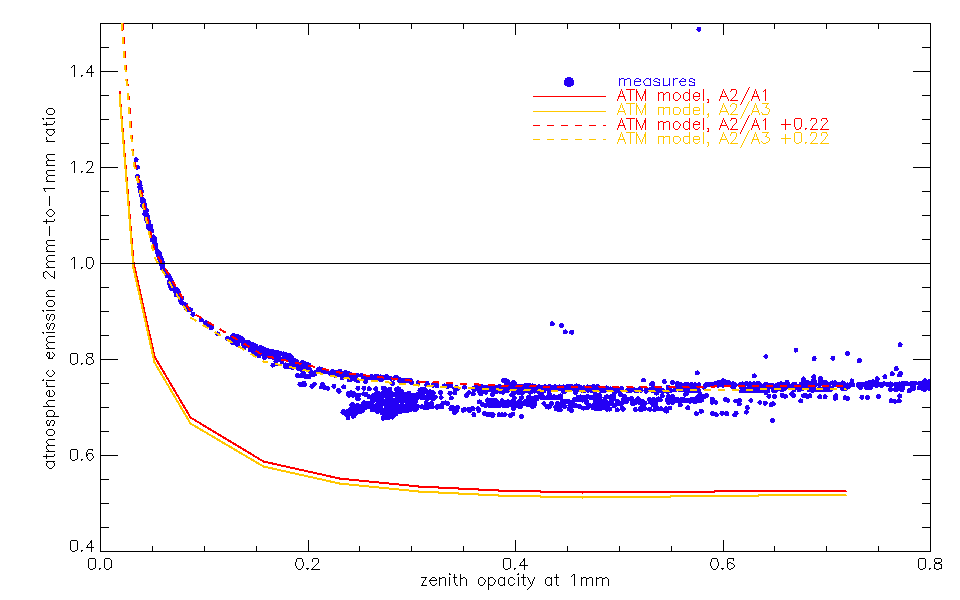
\includegraphics[width=0.9\textwidth]{Figures/opacity_tau1_tau2_emissionratio_N2R9_N2R10.png}
\caption{Ratio of the atmospheric emission in NIKA2 bands defined as
  in Eq.~\ref{eq:opacity_emission_ratio}, compared with the ATM-model
  predicted ratio calculated as in Eq.~\ref{eq:opacity_emission_ratio_model}}
  \label{fig:opacity_emission}
\end{center}
\end{figure}

The ratios between the 150 GHz and the 260 GHz NIKA2 zenith opacity
estimates, quoted $\tau_{2mm}$ and $\tau_{1mm}$ , and
between the NIKA2 $\tau$ and the IRAM taumeter values are presented in
Fig.~\ref{opacity_ratios}, along with the expectation values derived for NIKA2 bands
using the ATM model described in \ref{Pardo2002}. Namely, these
predicted values $\tau^{th}$ are calculated from the ATM-model
atmospheric zenith opacity $\tau^{ATM}$ using:  
\begin{equation}
  \tau^{th}_{A_i} = - \ln{\frac{\int e^{-\tau^{ATM}(\nu)}
      T_{A_i}(\nu) d\nu}{ \int T_{A_i}(\nu) d\nu}},
\end{equation}

where the NIKA2 bandpasses $T_{A_i}$ for arrays $A_i$, $i=1, 2, 3$, are the Martin-Pupplet reference transmissions
corrected by a Rayleigh-Jeans term  $T'_{A_i}(\nu) /
\left( \frac{\nu}{\nu_0}\right)^2$. 

In Fig.~\ref{fig:opacity_emission}, we
show the ratio of the atmospheric emission in NIKA2 bands defined as:
\begin{equation}
  R_{\rm{atm}} = \frac{1-e^{-\tau_{2mm}}}{1-e^{-\tau_{1mm}}}.
    \label{eq:opacity_emission_ratio}
\end{equation}

It is compared with the ATM-model predicted ratio
\begin{equation}
  R_{\rm{atm}}^{th} = \frac{\int (1 - e^{-\tau^{\rm{ATM}}}) T_{A_2}(\nu) d\nu }{\int T_{A_2}(\nu) d\nu} / \frac{\int (1 -
      e^{-\tau^{\rm{ATM}}}) T_{A_{1}}(\nu) d\nu }{\int T_{A_1}(\nu)
        d\nu} .
      \label{eq:opacity_emission_ratio_model}
\end{equation}

In Fig.~\ref{fig:opacity_errors}, we investigate different effects that can impact the precision with
which the zenith opacities are determined: the upper panel shows the
expected dispersion in the NIKA2 $\tau$ values coming from the transmission
measurement uncertainties: to higlight this effect, we consider a very
pessimistic relative uncertainty of $10\%$ (whereas $1\%$ would have
been a more realistic value), and the lower panel shows the impact of the
uncertainty on the fraction of oxygene in the atmosphere, which mainly 
translates in an uncertainty on the atmospheric absorption around
$118\, \rm{GHz}$: the nominal absorption predicted by the ATM model is
modified by a factor from 0.5 to 2 in the $117-120\, \rm{GHz}$
frequency band, where the $0_2$ contributions largely dominates the
water vapor ones. 



We have compared $C_0$ values, the resonance frequency at zero atmosphere,
between different runs. It appears to vary in a systematic manner. For example
we have compared N2R6 and N2R7. The change of frequencies when converted to
temperature (with $c_1$) is of about $25$ and $86$~K at 1 and $2$~mm. This
cannot be a real change of the background. Translated back by a median value
of $c_1$ ($=2500$ and $1500$~Hz/K at 1 and 2 mm), we obtain a 62.5 and 128 kHz
median downward shift of all resonant frequencies between N2R6 (October 2016)
and N2R7 (December 2016). The likely explanation is that of a slight ageing of
the KIDs. A single monolayer of oxyde could be enough to produce the downward
shift.



Only a fraction of the signal is transmitted by the atmosphere and
reaches NIKA2 detectors. 
The relation between uncorrected observed flux densities
$\tilde{S}_{\nu}$ and top-of-the-atmosphere flux densities $S_{\nu}$
is parametrized from the zenith opacity $\tau_{\nu}$
and the line-of-sight air mass $x$, such as
\begin{equation}
\tilde{S}_{\nu} = S_{\nu} \, e^{-\tau_{\nu} \cdot x}.
\label{eq:uncorr_flux}
\end{equation}

An accurate derivation of the opacity condition for each scan is
required in order to retrieve the source signal at the top of the
atmosphere. Opacity correction uncertainties even prevail in the
final calibration error budget (see Chapter~\ref{se:error}).

We developped three opacity derivation methods, which are discussed
in the sections below, and extensively tested their robustness against
observing condition. The 'taumeter' method discussed in
Sect~\ref{se:taumeter-method} relies on measurements provided by the
resident IRAM tau-meter operated at $225~\rm{GHz}$ and a fit of the
opacity estimates in NIKA2 frequency bands by imposing the flux
density stability against atmospheric condition. The 'skydip' method
described in Sect~\ref{se:skydip-method} consists in using NIKA2 as a
taumeter by resorting to a series of skydip scans, the selection of
which is addressed in Sect.~\ref{se:skydip-selection}. Finally, the
'corrected skydip' method presented in Sect.~\ref{se:corrected-skydip}
is a modifed version of the 'skydip' method that minimizes the
dependence of the measured flux density on the opacity.\\


Consistency check between two independent methods, the \emph{taumeter}-
and \emph{skydip}-based methods, constitutes a first
robustness test, which is addressed in this chapter.
Then, the opacity estimates in NIKA2 bands are
ultimately tested by assessing the stability of the
top-of-the-atmosphere flux densities for a large range of
atmsopheric conditions, as discussed in Chapter~\ref{se:photometry}.



%----------------------------------------------------------------------------------------
%	taumeter Method
%----------------------------------------------------------------------------------------
\section{Taumeter-based method {\color{blue} Laurence $\&$ Juan}}
\label{se:taumeter-method}

The IRAM 30m falicity is equipped of a resident taumeter, which performs
elevation scans at a fixed azimuth and is operated at 225~GHz, to
monitor the atmospheric opacity.
Time-stamped
zenith opacities at $225$~GHz $\hat{\tau}_{225}$ are derived from the
taumeter measures by Dave~L.~John. Two different $\hat{\tau}_{225}$
estimates are fitted, one relying on a linear model and the other on
an exponential fitting model. The $\hat{\tau}_{225}$ estimates are then
filtered using the cuts $0< \hat{\tau}_{225} <1.2$ and $R^2 > 0.99$, where
$R$ is the correlation coefficient between the two flavours of
$\hat{\tau}_{225}$ estimates. 

The time-stamped $\hat{\tau}_{225}$ estimates are sampled every
{\color{magenta} XXX secondes}, whereas the typical duration of NIKA2
observing scans is of several minutes. Thus we use median filtered
version of the $\hat{\tau}_{225}$ estimates. {\color{magenta} Juan to
complement/rewrite this paragraph}\\


\begin{figure}[ht!]
  \begin{center}
    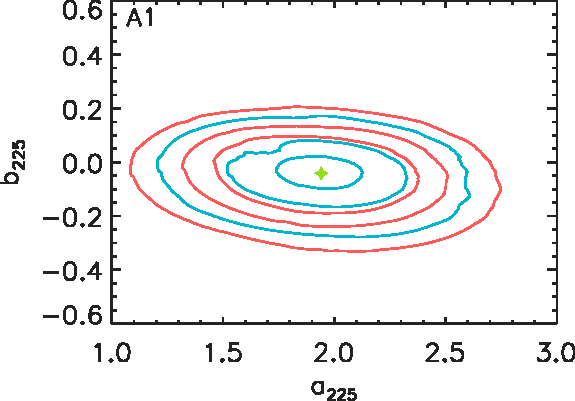
\includegraphics[clip=true, trim={0, -0.3cm, -0.3cm, 0}, width=0.4\textwidth]{Figures/Opacity/fit_nika2_tau_from_taumeter_mwc349_a1.pdf}
    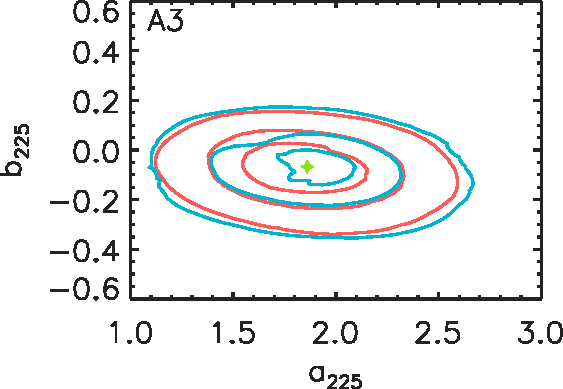
\includegraphics[clip=true, trim={0, -0.3cm, -0.3cm, 0}, width=0.4\textwidth]{Figures/Opacity/fit_nika2_tau_from_taumeter_mwc349_a3.pdf}
    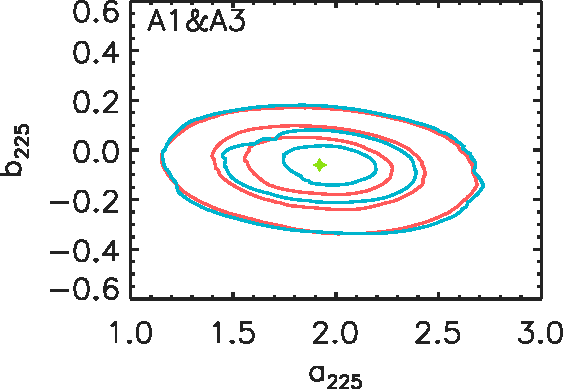
\includegraphics[clip=true, trim={0, -0.3cm, -0.3cm, 0}, width=0.4\textwidth]{Figures/Opacity/fit_nika2_tau_from_taumeter_mwc349_1mm.pdf}
    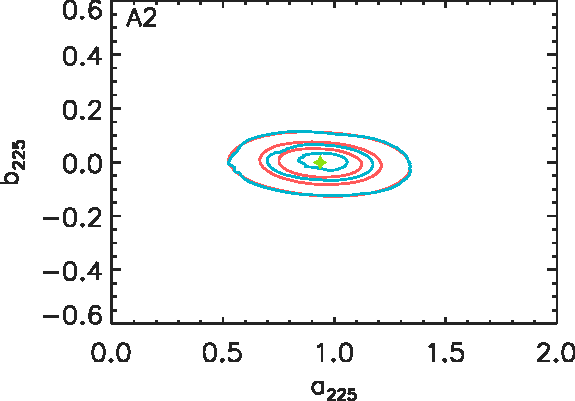
\includegraphics[clip=true, trim={0, -0.3cm, -0.3cm, 0}, width=0.4\textwidth]{Figures/Opacity/fit_nika2_tau_from_taumeter_mwc349_a2.pdf}
    \caption[IRAM taumeter to NIKA2 opacity model]{IRAM $225$GHz taumeter to
    NIKA2 opacity relation fit.
    The $a_{\nu}^{225}$ and
    $b_{\nu}^{225}$ parameter space is explored for Array 1 (upper left),
    Array 3 (upper right), the combination of 1mm arrays (lower left)
    and Array 2 (lower right).
    The red contours correspond to rms
    errors of the measured-to-median flux density ratio of $9\%$, $10\%$
    and $12\%$ at 1mm and $4.5\%$, $5\%$ and $6\%$ at 2mm. The blue
    contours are the $68$, $95$ and $99\%$ confidence
    level contours of the parameters estimated using the $\chi^2$
    minimization.
    The best fit values are shows as green stars} 
\label{fig:taumeter_fit}
\end{center}
\end{figure}

We fit the the relations between the IRAM
$225$GHz taumeter opacities and NIKA2 band pass opacities using
observation of calibration sources which spans a large range of air
masses. We use a series of 64 scans of MWC349, which consists of the
baseline selected sub-set of scans from the 68 available scans for
this source during N2R9.
It constitutes an homogeneous data set in flux density but
heterogeneous in atmospheric conditions: zenith opacities at $225$GHz
range from 0.08 to 0.32 and elevations from $23$ to $73$
degrees, spanning a large range of air mass as required. NIKA2 opacities
$\tau_\nu$, for $\nu$ corresponding
to Array 1, 2, 3 and the combination of Arrays 1 and 3, are estimated
from the $225$GHz taumeter median-filtered exponential-based opacity
estimates $\tau_{225}$ as
\begin{equation}  
  \tau_\nu =  a_\nu^{225}\tau_{225} + b_\nu^{225},          
\end{equation}
where the parameters $a_\nu^{225}$ and $b_\nu^{225}$ are fitted to ensure
that the non-corrected flux densities $\tilde{S}_\nu$ are stable againts
$\tau_{225}$ after correction of the atmospheric attenuation by
inversion of Eq.~\ref{eq:uncorr_flux} using 
\begin{equation}  
  S_\nu = \tilde{S}_\nu e^{(a_\nu^{225}\tau_{225} + b_\nu^{225}) \cdot x}.
  \label{eq:opacorr_taumeter}
\end{equation}

We tested two estimators of the flux stability. The first one relies
on minimising the
standard deviation of the measured-to-median flux densities ratio
after correction of the opacity using Eq.~\ref{eq:opacorr_taumeter}. The second
one consists in rewriting the rms minimisation as an unweighted
$\chi^2$ minimisation using:
\begin{equation}
\chi^2 = \sum_{i=1}^{N} \frac{1}{\sigma^2} \, \left( \frac{S_\nu}{Med(S_\nu)} -1 \right)^2,  
\end{equation}
where $\sigma$ is the rms error of the flux density estimates. Note
that these estimators do not depends on
the absolute scale of the flux density of the source.

Figure~\ref{fig:taumeter_fit} show the two flux-stability estimate
contours in the parameter plane ($a_\nu^{225}$, $b_\nu^{225}$), as
well as the best-fitting parameter values. We find
$a^{225} = [1.94,  1.86, 1.92]$ and $b^{225} = [-0.04,  -0.07, -0.06]$
for A1, A3, and the 1mm array combination, while $a^{225}=0.94$ and
$b^{225}=0$ for A2.   

% bf_a     = 1.9401878      0.94233333       1.8952941       1.9342579
% err_bf_a = 0.16605729     0.097230351     0.084799830      0.12000000
% bf_b     =  -0.045000000       0.0000000    -0.058426966    -0.055000000
% err_bf_b = 0.049497475     0.026340184     0.021199958   0.038890873
%
% -0.043488288  -0.00057861635    -0.060658083    -0.053333333
% 0.050634888     0.027028985     0.022710888     0.040069384
%
%$a = [1.94,  0.94,  1.86,  1.92]$
%$b = [-0.04, 0.00, -0.07, -0.06]$

As stated latter, we will use the 'taumeter' method as an alternative method
to correct for the atmospheric attenuation and perform consistency
checks for baseline results in Sect.~\ref{se:photometry_others}.




%----------------------------------------------------------------------------------------
%	skydip-based Method
%----------------------------------------------------------------------------------------
\section{Skydip-based method {\color{blue} Xavier $\&$ Laurence}}
\label{se:skydip-method}

% LP: copie de l'intro de Xavier
In NIKA2, the opacity is measured via a total-power technique, which was
successfully tested with NIKA. The details of this technique and its agreement
with the Atmospheric Transmission at Microwaves (ATM) model
(\cite{2001IEEE....49.1683C}) are described in \cite{Catalano:2014nml}. The
underlying idea is to replace the opacity, usually delivered by the resident
IRAM tau-meter by a measurement that uses the NIKA2 instrument itself
as a tau-meter. Using this procedure we can directly derive an opacity
integrated in the NIKA2 very bandpasses and in the same line-of-sight of the
source in the considered map. For that purpose, we assume that the resonance
frequency of each KID varies linearly with the total power. First, we have to
calibrate the relationship between total power and opacity. Then we can use
that calibration to measure the opacity during a given scan.
% fin copie

For each KID $k$, the absolute value of the resonance frequency
$f_{tone}^k$ moves with the atmospheric load according to

\begin{equation}
\ftone^k  = C_0^k - C_1^k T_{atm}[1-e^{-\tau/\sin\delta}]
\label{eq:skydip}
\end{equation}

%FXD corrected 
%{\bf LP: pourquoi signe plus alors qu'on utilise un signe moins dans
%  Eq. 2 du papier instru ?}

where $C_0^k$ is a constant equal to the resonance
frequency at zero opacity, $C_1^k$ is the calibration conversion
factor in kHz$/$K, $T_{atm}$ is the equivalent temperature
of the atmosphere (taken as a constant at 270~K), $\tau$ the zenith
opacity and $\delta$ the average elevation of the telescope.
By assuming a homogeneous plane-parallel atmosphere, the airmass $x$ is defined from the
elevation as $x = \left(\sin\delta\right)^{-1}$. 

The coefficients $C_0^k$ and $C_1^k$ are expected to be constant in
time within at least a cooldown cycle, and are determined using a {\emph
skydip} procedure. This consists in moving the telescope in elevation
step by step, that is performing a skydip scan, as
defined in~Sect.~\ref{se:skydip}, and monitoring, for each kid, the
evolution of $\ftone^k$ versus the air mass and to fit the zenith
opacity $\tau$ and $C_0^k$ and $C_1^k$. The acquisition time spend on each
elevation step, which is of about twenty seconds, is chosen to reduce
the error in the determination of $\ftone^k$.

All skydips, obtained under various opacity
conditions, are analysed together to break the degeneracies between
the opacity and the responsivity ($C_1^k$). The procedure has two steps.
First, all the skydips are analysed individually to simply extract
$\ftone^k$ for each stable elevation. Secondly, a simultaneous fit is done
for all 
parameters ($\tau$, $C_0^k$ and $C_1^k$.)
Error bars on $\tau$ are estimated by doing
this procedure on blocks of 40 kids only and getting a dispersion on the
resulting $\tau$ from the different blocks. Usually the dispersion comes out as
$4\times 10^{-3}$ at 1 mm and $1\times 10^{-3}$ at 2 mm. Once the $\tau$ values
are estimated for each skydip (as the average over the blocks), we compute
(while fixing $\tau$) the $C_0$ and $C_1$ final values for each KID. We thus
retrieve the coefficients of all the KIDs even though some of them could not
contribute to the $\tau$ determination.

We observe that the skydip-fitted $\tau$ values are, as expected, common
between different detectors of the same array. By comparing the results of different skydips, we
have verified experimentally that the coefficients $C_0$, $C_1$ are stable,
within the fit errors, on very long time scales within a cooldown cycle. The
coefficients can thus be applied to the whole observing campaign in order to
recover the opacity of each scan.
\noindent {\bf FM : a figure would help to convince the reader that it is stable on lng time
 scale, which is a key point.}\\ {\color{magenta} FXD: I will do that figure}

The skydip-based procedure consists in fitting a couple of paramaters ($C_0$,
$C_1$) for each of the several thousand valid KIDs. This requires to
have on hands a sizable amount of skydip scans -- typically ten to
twenty -- that i) span the whole opacity range and ii) avoid hightly
perturbated atmosphere to met the plane-parallel atmosphere
assumption. To that aim, we recommand to perform a skydip scan twice a
day during a scientific campaign. Then the ($C_0$, $C_1$)
determination process relies on a selection of the skydip scans.




%----------------------------------------------------------------------------------------
%	skydip selection
%----------------------------------------------------------------------------------------
\section{Skydip selection {\color{YellowGreen} Laurence}}
\label{se:skydip-selection}

\begin{figure}[ht!]
\begin{center}
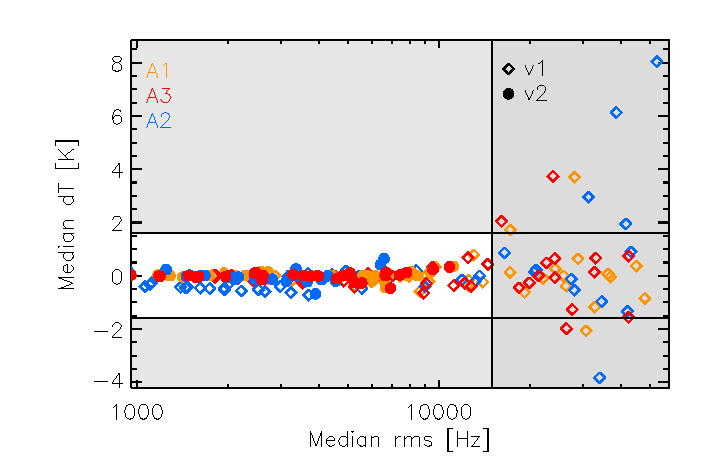
\includegraphics[clip=true,width=0.8\textwidth]{Figures/Opacity/plot_skydip_selection_two_crit.pdf}
\caption[N2R9 skydip scan selection.]{ Median dT quality-fit criterion is plotted in fonction of Median rms criterion for each skydip scans of the N2R9 campaign and for the three arrays. Both criteria are nicely correlated. Empty diamonds show the results of the first iteration of the skydip coefficient estimation, whereas filled circled show the second iteration, for which only the skydips that met both fit-quality criteria are included. After the second iteration, all the remaining skydips met the criteria.}
\label{fig:skydipselection}
\end{center}
\end{figure}

For each skydip scan and for each bunch of 40 KIDs, we compute the
difference between the measured KID resonance frequency and the model
given in Eq.~\ref{eq:skydip} taken at the best-fit values of the
($C_0$, $C_1$) parameters. Then we determine two indicators
of the fit quality per skydip. First, the standard deviation of the
measure-to-model difference is calculated over all the KIDs in a
bunch. For each skydip, we evaluate the median rms, which is the
median over the KID bunches of the standard deviation per bunch, given
in Hz. Secondly, for each scan, we compute the average
measure-to-model difference of each KID $k$, labelled $dT_k$, which is
then converted from Hertz to Kelvin using the $C_1$ parameter of the
KID $k$. Median $dT$ is the median of $dT_k$ over all the KID of an
array. With these two indicators in hands, we discard the skydip scans
that are noisy or that yield a poor fit by applying the selection
criteria

\begin{itemize}
\item Median $\rm{rms} < 1.5 \times 10^{4}~\rm{Hz}$
\item Median $dT < 1.6~\rm{K}$
\end{itemize}

The threshold values have been determined using the set of 44 skydip
scans of N2R9. The Median rms cut corresponds to twice the median of
this quantity per skydip scan, whereas the Median $dT$ cut is twice
the standard deviation of Median $dT$ over the skydips.
N2R9 skydip scan selection is illustrated in
Fig.~\ref{fig:skydipselection}, in
which the agreement between the two fit-quality criteria is clearly
seen. The ($C_0$, $C_1$) estimation proceeds in two steps: first the
parameters are estimated using all the available skydip scan for a
given campaign, then the estimation is re-iterated using the only
skydip scans that met the fit-quality criteria. After the second
iteration, we check that no extra skydip outlier are left, as shown by
the 'v2' label data points in Fig.~\ref{fig:skydipselection}. After
selection of the skydip scans acquired during the N2R9 campaign, 15
skydips are kept for the final step of the ($C_0$, $C_1$) fit. 


\begin{figure}[ht!]
  \begin{center}
    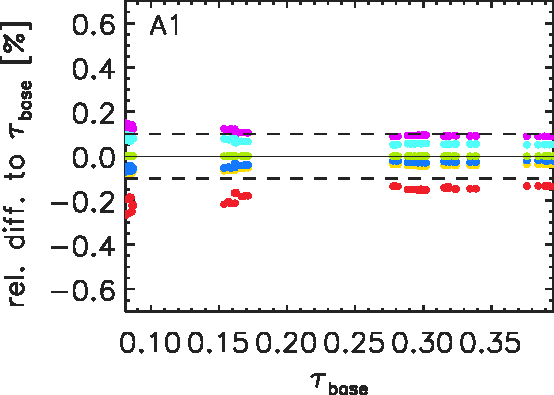
\includegraphics[clip=true, trim={0, -0.3cm, -0.3cm, 0},  width=0.42\textwidth]{Figures/Opacity/Skydip_selection_impact_a1.pdf}
    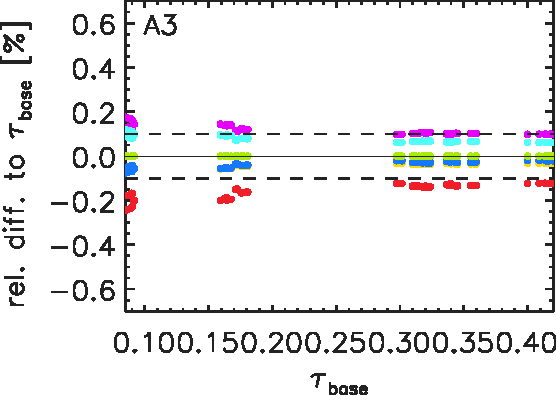
\includegraphics[clip=true, trim={0, -0.3cm, -0.3cm, 0},  width=0.42\textwidth]{Figures/Opacity/Skydip_selection_impact_a3.pdf}
    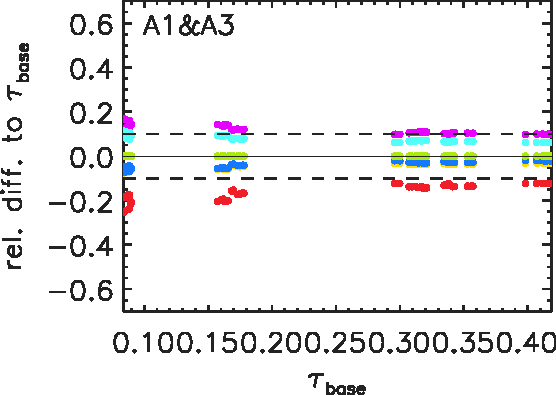
\includegraphics[clip=true, trim={0, -0.3cm, -0.3cm, 0},  width=0.42\textwidth]{Figures/Opacity/Skydip_selection_impact_1mm.pdf}
    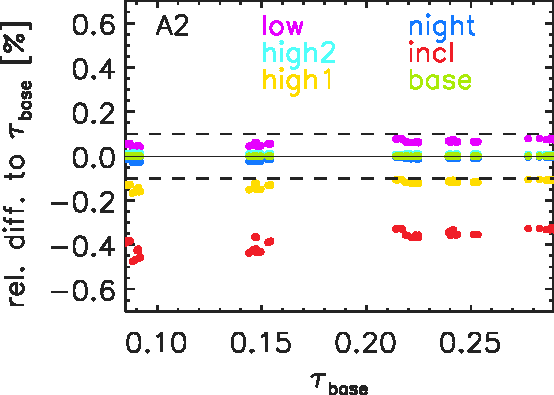
\includegraphics[clip=true, trim={0, -0.3cm, -0.3cm, 0},  width=0.42\textwidth]{Figures/Opacity/Skydip_selection_impact_a2.pdf}
   \caption[Skydip selection impact on opacities]{Skydip-selection
    impact on the opacity estimates. For a series of calibration scans
    of MWC349 acquired during N2R9, the relative difference
    w.r.t. the baseline opacities $\tau_{\rm{base}}$ (labeled 'base')
    are shown as a function of $\tau_{\rm{base}}$ for five skydip
    selections. The most inclusive one (labeled 'incl')
    includes 38 skydips of the 44 available. 'night' comprizes 11
    skydips acquired during nighttime. 'low' consists of 20 skydips
    acquired in low opacity conditions. 'high
    1' and 'high 2' are fit-quality based selections relying of relaxed
    ('high1') or tighened ('high 2') criteria w.r.t. the baseline
    criteria given in Sect.~\ref{se:skydip-selection}. The dashed
    lines figure a $10\%$ opacity difference
    w.r.t. $\tau_{\rm{base}}$. } 
\label{fig:skydip-selection-impact}
\end{center}
\end{figure}


We test the stability of the ($C_0$, $C_1$) parameters against the
exact choice of the selection criteria.
We derive ($C_0$, $C_1$) parameter sets for the N2R9 campaign using
six skydip selections: the baseline selection (labeled 'base')
consists in the fit-quality based selection described above, which
comprizes 15 skydips, the selection labeled 'incl' consists of an
inclusive selection of 38 skydips in which only the noisier ones were
discarded, the 'night' selection comprizes 11 skydips acquired during
between 21:00 and 09:00 UT,
'high 1' and 'high 2' are two different selections, which comprize 23
and 13 skydips and are based on fit quality criteria that are
respectively relaxed or tighened with respect to the baseline criteria, 
and 'low' corresponds to a selection of 20 skydips acquired while
$\tau_{1mm} < 0.44$. Each ($C_0$, $C_1$) sets are used to derive
zenith opacity of the N2R9 calibration scans of MWC349. 
Figure~\ref{fig:skydip-selection-impact} shows the relative
difference between each $\tau$ estimates and the baseline $\tau$
estimates as a function of the baseline $\tau$. The relative
differences are basically constant for the whole opacity range: the
main effect of the skydip selection is a normalisation factor on the
$\tau$ estimates at both wavelength. At both wavelength, this factor
is below $10\%$ of the baseline $\tau$ for most of the skydip
selections. However, this is of about $10\%$ for the 'low' selection,
which highlight the necessity of including good skydips acquired in
high $(\tau_{1\rm{mm}} > 0.44)$ opacity conditions in the final
selection. The 'incl' (inclusive 38-skydip based) selection results in the larger
difference w.r.t. the baseline $\tau$, which are up to $20\%$ at 1mm
and up to $40\%$ at $2$mm, whereas the 'high 1' (mild quality-fit)
selection suffices to reduce the relative difference below $10\%$ at
1mm and below $15\%$ at 2mm.
As a summary, the $\tau$ estimates are robust against the exact skydip
selection as long as the selection includes good
skydips in high opacity condition $(\tau_{1\rm{mm}} > 0.44)$ and as the poor
fitting skydips are excluded. When these conditions are met, the
skydip selection induced uncertainties are below $10\%$ at 1mm and
below $15\%$ at 2mm. 

We conclude that opacities at both wavelengths can be reliably
estimated from a series of skydip scans using the (C0, C1) model.


%We conclude that opacities at 1mm can be reliably estimated from a series of skydip scans using the (C0, C1) model. %By contrast, for the 2mm opacities, a skydip-based method is not stable enough against the skydip selection. Thus, we adopt an hybrid approach. 

%\section{The hybrid method}

%The hybrid method comprizes two-steps: i) first the 1mm opacities,
%that are $\tau_{A1}$ and $\tau_{A3}$, are determined using the skydip
%method described in Sect.~\ref{se:skydip-method}, ii) then the 2mm
%opacity $\tau_{A2}$ is extrapolated from the 1mm ones using a modified
%ATM model. Namely, for the second step, we perform:

%\begin{equation}
%\tau_{A2} = \left( \left.\frac{\tau_{A2}^{\rm{ATM}}}{\tau_{A3}^{\rm{ATM}}}\right\vert_{\tau_{A3}} + \alpha \right) \tau_{A3},
%\end{equation}

% where $\alpha$ is an offset, which are estimated from the observations themselves, and the ratio is the predicted zenith opacity ratio for A2 and A3 frequency bands using the ATM model described in \ref{Pardo2002} and taken at the measured A3 zenith opacity. The zenith opacity expectations for the array $A_i$ is
%\begin{equation}
%  \tau^{\rm{ATM}}_{A_i} = - \ln{\frac{\int e^{-\tau^{ATM}(\nu)} T_{A_i}(\nu) d\nu}{ \int T_{A_i}(\nu) d\nu}},
%\end{equation}
%where the bandpasses $T_{A_i}$ for arrays $A_i$, $i=1, 2, 3$, are the Martin-Pupplet reference transmissions
%corrected by a Rayleigh-Jeans term  $T'_{A_i}(\nu) / \left( \frac{\nu}{\nu_0}\right)^2$. 

%We observe that the measured \emph{shape} of the measured opacity ratio is well described by the ATM expectations whereas its \emph{amplitude} is too low by an offset $\alpha$, which we dertermine using a data-driven approach. We estimate $\alpha$ as the offset that ensures a stability of the A2 flux over the whole opacity span.  

%\addparag{$\alpha$ fit + FIG}


%----------------------------------------------------------------------------------------
%	skydip opacity tests
%----------------------------------------------------------------------------------------
\section{Skydip-based opacity measurements and tests {\color{blue} Laurence}}
\label{se:skydip-opacity_tests}

We perform basic sanity tests of the skydip-based opacity
measurements, referred to as 'skydip' opacities hereafter.
First, we test the stability of the 'skydip' opacities from one
observation campaign to another.
Figure~\ref{fig:skydip-to-taumeter-correl} shows the
correlation between the 'skydip' $\tau$ estimates $\tau_{\rm{skydip}}$
and the taumeter zenith opacities $\tau_{225}$ for a series of scans
of Uranus and MWC349 acquired during three campaigns. As guidelines,
we also show the predicted correlations using an ATM model integrated
in NIKA2 wavebands. At 1~mm, the
$\tau_{\rm{skydip}}$ to $\tau_{225}$ correlation relations are
consistent for the three campaigns. They are
also in agreement with the ATM model expectations. At 2~mm, more
dispersion is observed between each correlation relations although
they are compatible with each others within statistical errors.
We note that the ATM model underestimates the
measured $\tau_{\rm{skydip}}$. This mild discrepancy with the
ATM model predictions is yet to be understood, but has no impact on
our opacity measurements, which do not rely on any ATM model nor on
the precision with which the observing bandpasses are known.


\begin{figure}[ht!]
  \begin{center}
    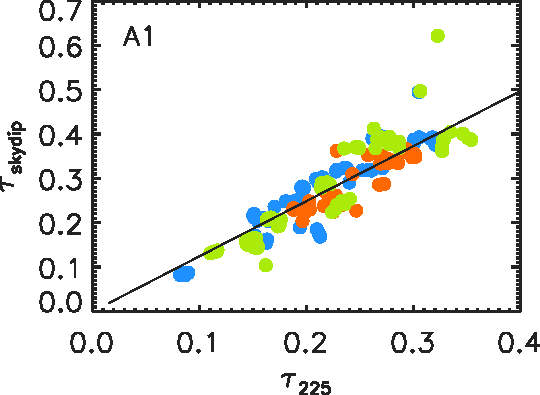
\includegraphics[clip=true, trim={0, -0.3cm, -0.3cm, 0}, width=0.42\textwidth]{Figures/Opacity/Opacity_correl_skydip_vs_tau_a1.pdf}
    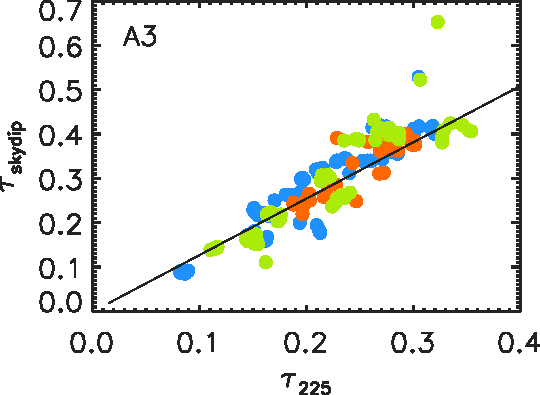
\includegraphics[clip=true, trim={0, -0.3cm, -0.3cm, 0}, width=0.42\textwidth]{Figures/Opacity/Opacity_correl_skydip_vs_tau_a3.pdf}
    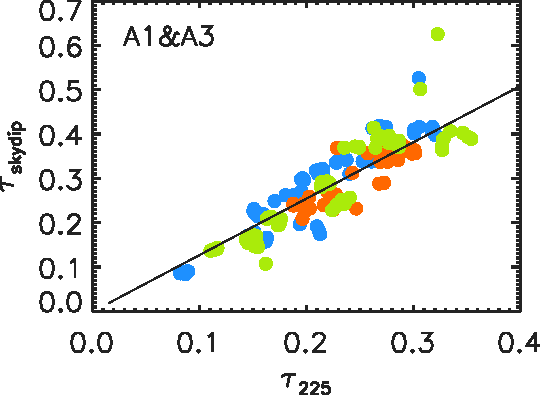
\includegraphics[clip=true, trim={0, -0.3cm, -0.3cm, 0}, width=0.42\textwidth]{Figures/Opacity/Opacity_correl_skydip_vs_tau_1mm.pdf}
    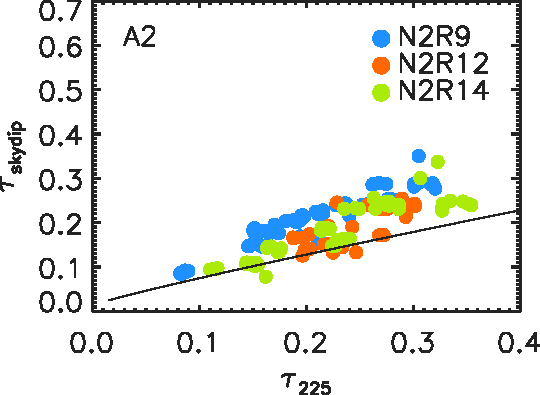
\includegraphics[clip=true, trim={0, -0.3cm, -0.3cm, 0}, width=0.42\textwidth]{Figures/Opacity/Opacity_correl_skydip_vs_tau_a2.pdf}
   \caption[NIKA2 skydip-based vs taumeter opacities]{ NIKA2
    skydip-based opacities vs IRAM 225GHz taumeter opacities. The
    modeled correlations relying on an ATM model integrated in NIKA2
    bands are shown in black.} 
\label{fig:skydip-to-taumeter-correl}
\end{center}
\end{figure}

We check the robustness of the 'skydip' $\tau$ againts the
observing elevation. 
Figure~\ref{fig:skydip-to-taumeter-ratio-vs-elev} shows the ratio of NIKA2
'skydip' opacities to the $225$GHz taumeter opacities as a function of
the observing elevation.

\begin{figure}[ht!]
  \begin{center}
    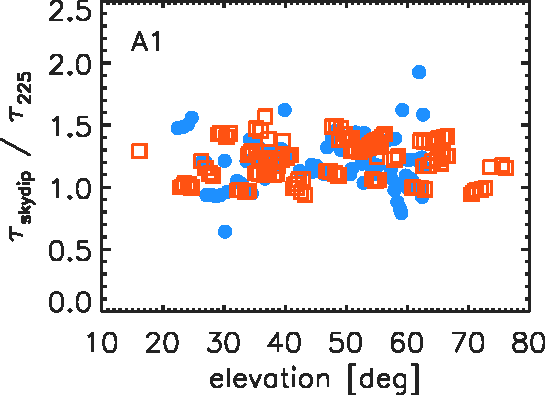
\includegraphics[clip=true, trim={0, -0.3cm, -0.3cm, 0}, width=0.42\textwidth]{Figures/Opacity/Opacity_skydip_to_taumeter_vs_elev_a1.pdf}
    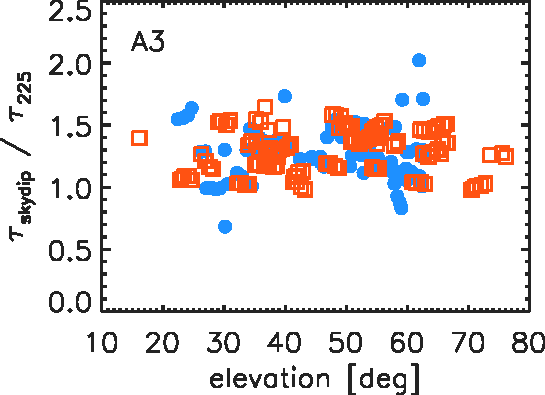
\includegraphics[clip=true, trim={0, -0.3cm, -0.3cm, 0}, width=0.42\textwidth]{Figures/Opacity/Opacity_skydip_to_taumeter_vs_elev_a3.pdf}
    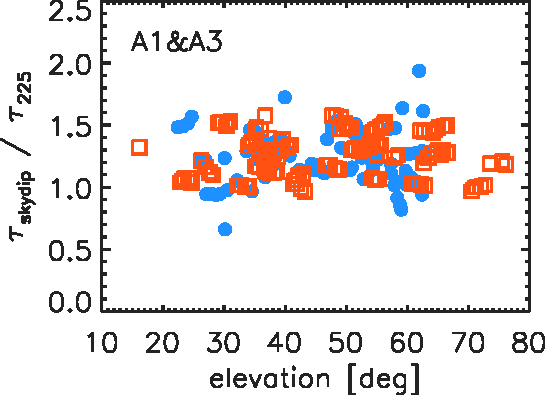
\includegraphics[clip=true, trim={0, -0.3cm, -0.3cm, 0}, width=0.42\textwidth]{Figures/Opacity/Opacity_skydip_to_taumeter_vs_elev_1mm.pdf}
    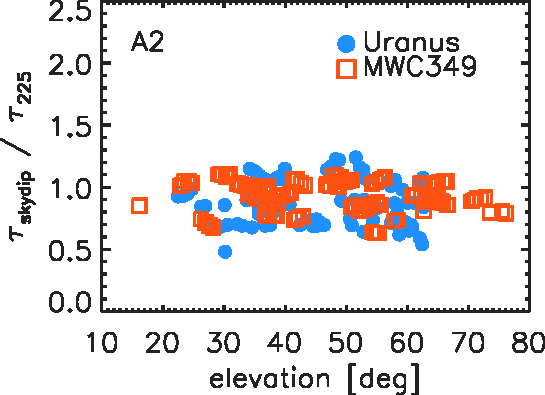
\includegraphics[clip=true, trim={0, -0.3cm, -0.3cm, 0}, width=0.42\textwidth]{Figures/Opacity/Opacity_skydip_to_taumeter_vs_elev_a2.pdf}
    \caption[NIKA2 skydip-based opacity stability against observing elevations]{NIKA2
    skydip-based opacities stability againts the observing elevation.} 
\label{fig:skydip-to-taumeter-ratio-vs-elev}
\end{center}
\end{figure}



%----------------------------------------------------------------------------------------
%	Corrected skydip method
%----------------------------------------------------------------------------------------
\section{Corrected skydip method {\color{blue} Laurence}}
\label{se:corrected-skydip}

%%%%%%%%%%%%%%%%%%%%%%%%%%%%%%%%%%%%%%%%%%%%%%%%%%%%%%%%%
% 1-params correction
%%%%%%%%%%%%%%%%%%%%%%%%%%%%%%%%%%%%%%%%%%%%%%%%%%%%%%%%%%
We use the flux stability estimators described in
Sect.~\ref{se:taumeter-method} to fit a correction to the 'skydip'
opacities $\tau_{\rm{skydip}}$ as
\begin{equation}  
  \tau_\nu =  a_\nu^{\rm{skydip}}\tau_{\rm{skydip}}.        
\end{equation}

We find $a_\nu^{\rm{skydip}}$ of
$1.36 \pm 0.04$,
$1.23 \pm 0.02$,
$1.27 \pm 0.03$ and
$1.03 \pm 0.03$ for A1, A3, A1$\&$A3 and A2 respectively.
% a   = 1.3600000       1.0318470       1.2326556       1.2660000
% s_a = 0.038587182     0.028553570     0.019324699     0.026832816


%%%%%%%%%%%%%%%%%%%%%%%%%%%%%%%%%%%%%%%%%%%%%%%%%%%%%%%%%
% 2-params correction
%%%%%%%%%%%%%%%%%%%%%%%%%%%%%%%%%%%%%%%%%%%%%%%%%%%%%%%%%%
\begin{figure}[ht!]
  \begin{center}
    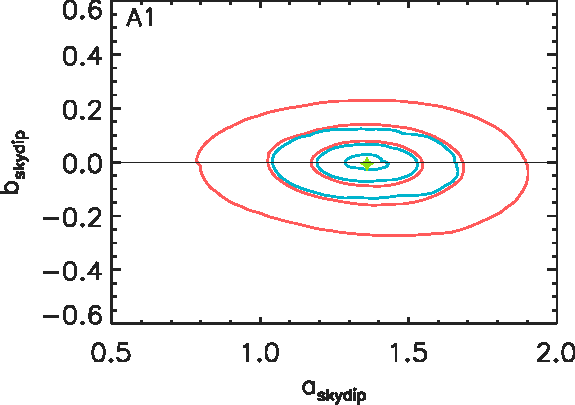
\includegraphics[clip=true, trim={0, -0.3cm, -0.3cm, 0}, width=0.42\textwidth]{Figures/Opacity/fit_nika2_tau_from_skydip_mwc349_a1.pdf}
    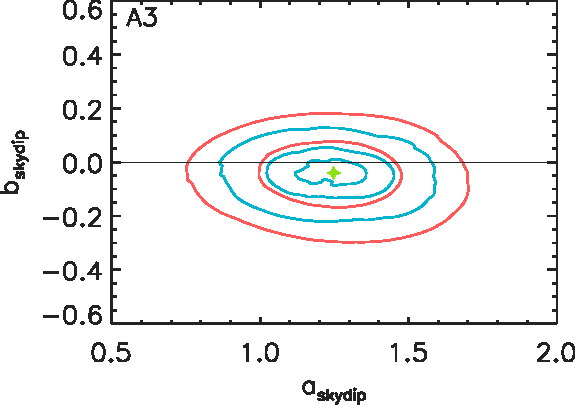
\includegraphics[clip=true, trim={0, -0.3cm, -0.3cm, 0}, width=0.42\textwidth]{Figures/Opacity/fit_nika2_tau_from_skydip_mwc349_a3.pdf}
    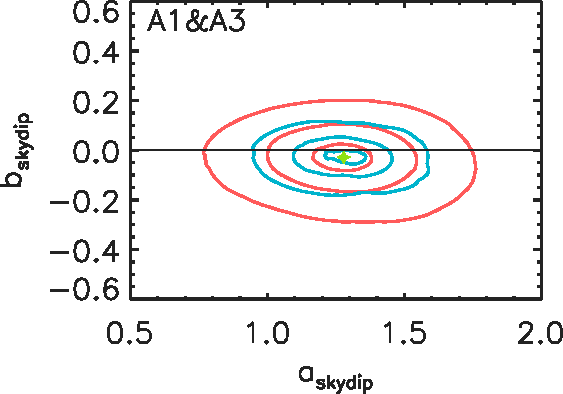
\includegraphics[clip=true, trim={0, -0.3cm, -0.3cm, 0}, width=0.42\textwidth]{Figures/Opacity/fit_nika2_tau_from_skydip_mwc349_1mm.pdf}
    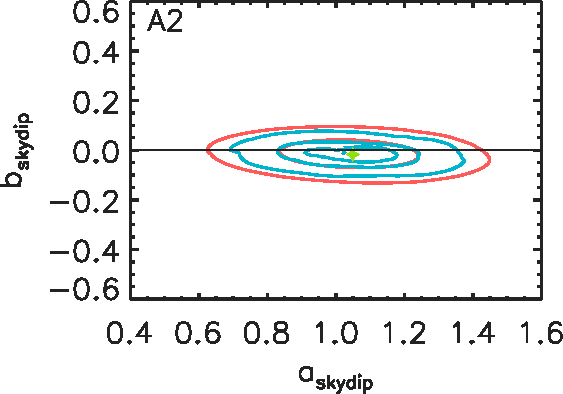
\includegraphics[clip=true, trim={0, -0.3cm, -0.3cm, 0}, width=0.42\textwidth]{Figures/Opacity/fit_nika2_tau_from_skydip_mwc349_a2.pdf}
    \caption[NIKA2 skydip-based opacity correcting
    relation]{Fit of the skydip-based opacity correcting relation
    parameters.
    The flux-stability estimator contours are shown in the plan
    $a_{\rm{skydip}} \equiv a_\nu^{\rm{skydip}'}$ and
    $b_{\rm{skydip}} \equiv b_\nu^{\rm{skydip}'}$
    for A1, A3, A1$\&$A3 and A2.
    The red contours enclose rms
    errors of the measured-to-median flux density ratio of $5.5$, $7$
    and $10\%$ at 1mm and $2.7$, $3.5$ and $5\%$ at 2mm. The blue
    contours correspond roughthly to the $68\%$, $95\%$ and $99\%$
    confidence levels drawn from the $\chi^2$ estimates.
    The best fit values are shows as green stars. Offset
    $b_\nu^{\rm{skydip}'}$ are compatible with zero within the $68\%$
    CL contours.} 
\label{fig:skydip_fit}
\end{center}
\end{figure}

Moreover, we test for an offset $b_\nu^{\rm{skydip}'}$ in the
correcting relation of the 'skydip' opacities as 
\begin{equation}  
  \tau_\nu =  a_\nu^{\rm{skydip}'}\tau_{\rm{skydip}} + b_\nu^{\rm{skydip}'}.      
\end{equation}
We repeat estimating the parameters of the correcting
relation. Confidence level contours in the parameter plan using the
two stability estimators are skown in Fig.~\ref{fig:skydip_fit}, as
well as the
best-fitting parameter values.
We find the best-fit $a_\nu^{\rm{skydip}'}$ estimates of
$1.36 \pm 0.04$,
$1.25 \pm 0.07$,
$1.28 \pm 0.04$ and
$1.05 \pm 0.05$ for A1, A3, A1$\&$A3 and A2 respectively, which are in
agreement with the best-fit values estimated using the single-parameter
correcting relation, whereas the best-fit values of the offsets
$b_\nu^{\rm{skydip}'}$ are compatible with zero at both wavelengths.
% a   = 1.3600000       1.0467126       1.2476650       1.2792013
% s_a = 0.037853031     0.050552977     0.068354972     0.044088207
% b   = -0.0053333333    -0.014432990    -0.040000000    -0.030731707
% s_b = 0.011925696     0.012184154     0.030641294     0.020823168


